\documentclass[11pt]{article}
\usepackage[brazilian]{babel}
\usepackage[utf8]{inputenc} %Deixa eu colocar letras com ascentos
\usepackage[T1]{fontenc}
\usepackage{amsmath}
\usepackage{color}
\usepackage{graphicx}


\title{Relatório - EP Fase 2 \\ Laboratório de Programação 2}



\begin{document}

\maketitle

\section{Integrantes}

\begin{itemize}

\item Victor Sanches Portella - Nº USP: 7991152

\item Lucas Dário - Nº USP: 7990940

\item Ruan Costa - Nº USP: 7990929

\end{itemize}

\section{Introdução}

Neste relatório temos como objetivo dar uma explicação concisa sobre a organização das classes no funcionamento do programa atualmente. Para isso, explicaremos o funcionamento do progrmaa inteiro, e iremos nos aprofundar nos assuntos que forem necessários.


\section{Funcionamento}

Nessa fase o EP ainda não têm o funcionamento de um jogo em si, mas já é possível ver diversos robos agindo em paralelo. Para isso, o script em Perl\footnote{Explicação do mesmo feita mais a frente} traduz diversos programas para um arquivo chamado \textbf{\color{red}Main.java}. 

Todos os robôs traduzidos serão colocados no mesmo time. Ao rodar o programa, os programas de cada robô será executado até o fim. Quando todos os robos tiverem acabado de executar, o programa será finalizado.

Cada robô imprime as instruções que execultou para que seja possível que nós possamos acompanhar a execução de cada robô.

\section{Classes}

\subsection{Classe Arena}


Essa classe representa a Arena em si. Nela, temos os seguintes atributos:

\begin{itemize}

	\item \textbf{Mapa}: Objeto do tipo \textbf{\color{red}Mapa} que representa o mapa em si. Nesse objeto existe uma matriz de Terrenos, cada um contendo informações como robôs naquele terreno, assim como cristais, bases, etc. Melhores explicações sobre esse objeto serão dadas mais a frente.
	
	\item \textbf{List<{\color{red}Robos}>}: Objeto do tipo \textbf{\color{red}List} usado como uma lista de objetos do tipo \textbf{\color{red}Robo}. Essa lista contêm todos os robos em jogo.
	
	\item \textbf{Tempo}: Uma variável inteira representando o número de rodadas já passadas. O valor inicial dessa variável é 0 e, a cada rodada, é incrementada em 1.

\end{itemize}

Principais métodos dessa classe:

\begin{itemize}

\item \textbf{Arena({\color{red}Mapa})}: Construtor da classe. Recebe uma mapa, e retorna uma arena vazia, ou seja, com nenhum robo, o tempo é iniciado com 0, e o mapa passado é definido como o mapa da arena.

\item \textbf{{\color{red}void} atualiza()}: Função que faz a Arena executar uma rodada. Atualmente, essa função percorre a lista de robôs de forma aleatória, executando em cada robô uma instrução de máquina. Em caso de conflito de instruções, tem preferência o robô que for executado primeiro naquela iteração.

\item \textbf{{\color{red}void} sistema({\color{red}Operacao})}: Função chamada pelos robôs para fazerem chamadas ao sistema. Toda vez que os robôs tentam executar uma ação que influencia seu exterior, ele só pode fazê-lo chamando esse método. O objeto do tipo \textbf{\color{red}Operacao} recebido descreve qual operacao está sendo executada, e qual objeto Programável está tentando executar aquela ação. Dependendo da operação, esse método mexe na pilha do robo, e executa as ações pedidas, caso possível.

\item \textbf{{\color{red}void} insereExercito({\color{red}Programa[ ]},{\color{red}Posicao[ ]},{\color{red}int})}: Função para inserir um exército de robôs na Arena. Para isso, recebe três argumentos:
		\begin{itemize}
			
			\item[+] \textbf{Programa[ ]}: Um vetor de objetos do 				tipo {\color{red}Programa}. Para cada programa, será criado um robô a ser inserido na Arena.
			
			\item[+] \textbf{Posicao[ ]}: Um vetor com posições x,y 				indicando onde cada robô criado deve ser posicionado, 				seguindo a odem do vetor de programas.
			
			\item[+] \textbf{{\color{red}int} time}: Um inteiro que 				indica a qual time esse exército pertencerá.  			
			
		\end{itemize}				

\end{itemize}


\subsection{Classe Maquina}

Um objeto da classe Máquina possui os seguintes atributos:
\begin{itemize}

\item \textbf{dados}
	Objeto do tipo Pilha. É a pilha de dados da maquina.
\item \textbf{mem}
	Vetor de Empilhaveis usado para o robo armazenar constantes.
\item \textbf{prog}
	Objeto do tipo Programa. É o vetor de comandos que aquela máquina executará.
\item \textbf{vars}
	Objeto do tipo variáveis. Guarda o estado atual das váriaveis de determinada máquina.
\item \textbf{arena}
	Referência para a Arena para a realização de chamadas ao sistema.
\item \textbf{index}
	Inteiro que guarda o índice do próximo comando do programa a ser executado.
\item \textbf{obj}
	Objeto do tipo Programável. À princípio é apenas uma referência para o robô que contém aquela máquina.
\end{itemize}


Principais métodos:

\begin{itemize}

	\item \textbf{Construtor}: Recebe o sistema (arena) com o qual a máquina vai se comunicar e o Programável que a possuíra.
				Mais uma vez, nesse ep, Programaveis são sempre robos. Inicializa mem com tamanho 10 e index setado em 0(zero).
	Funções mais importantes:
		void executaProx(): executa o comando cmd da posição index do programa. Para isso chama a função executaCmd(cmd), caso o programa já não tenha chegado ao fim.
		
	\item \textbf{{\color{red}int} executaCmd({\color{red}Comando})}: Executa o comando passado como argumento. Verifica  qual o código do comando e realiza a devida ação.
									 Retorna o índice do pŕoximo comando a ser lido. O sistema é chamado por meio da função sistema(), caso o comando passado precise de permissão da arena(i.e, se for ATK, COLLECT, DROP ou WALK).

	\item \textbf{{\color{red}void} sistema({\color{red}Comando})}:	 Pede para o sistema executar o Comando cmd.

		As outras funções são, em geral, auxíliares e estão bem explicadas nos comentários.

\end{itemize}

\subsection{Classe Mapa}

Essa classe é usada para representar o mapa que, em linhas gerais, é uma matriz hexagonal de objetos do tipo \textbf{\color{red}Terreno}. Nessa classe, temos 3 atributos: \textbf{\color{red}altura},\textbf{\color{red}largura} e uma matriz de objetos do tipo \textbf{\color{red}Terreno}.

Os métodos dessa classe estão bem explicados ja no código.

Para transformar a matriz normal em uma matriz hexagonal, tratamos ela assim como mostrado na imagem a seguir. Assim, apesar da matriz ser a usual, com a altura e largura definidas no atributo, usamos ela como uma matriz hexagonal através dos métodos da classe.

\begin{figure}[h]

    \center

    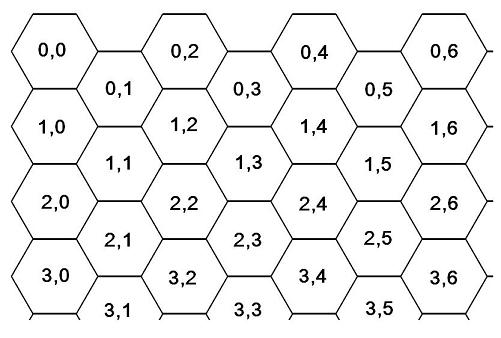
\includegraphics[width=10cm]{hex_array.jpg}

    \label{hexmatrix}

    \caption{Imagem mostrando o modo de enumeração dos terrenos}

\end{figure}

\subsection{Classe Programa}

\section{Interfaces}

\section{Tradutor em Perl}

\end{document}
